\chapter{Tesztek laborkörülmények között}

\section{A kísérleti rendszer}
Az elméleti eredmények validálásához elkészítettem egy szoba kicsinyített modelljét. Ez egy kartondobozban kapott helyet. A doboz hőtároló képessége elég csekély, ezért extra hőtároló tömegeket helyeztem bele, OSB falapot és egy elektromos kályhából vett samott téglát.
A fűtési teljesítményt halogén izzókkal juttattuk a rendszerbe. Ezek teljesítménye szabályozható, így ez a bemenet lineáris a szelepekkel ellentétben, azaz kétszer nagyobb beavatkozójelre kétszer nagyobb teljesítmény kerül a rendszerbe.
A hőmérsékletet mérjük a dobozban és azon kívül is. Zavarásként a mérőszoba ablakát kinyitjuk, így a doboz környezeti hőmérséklete lecsökken.

\begin{figure}[H]
	\centering
	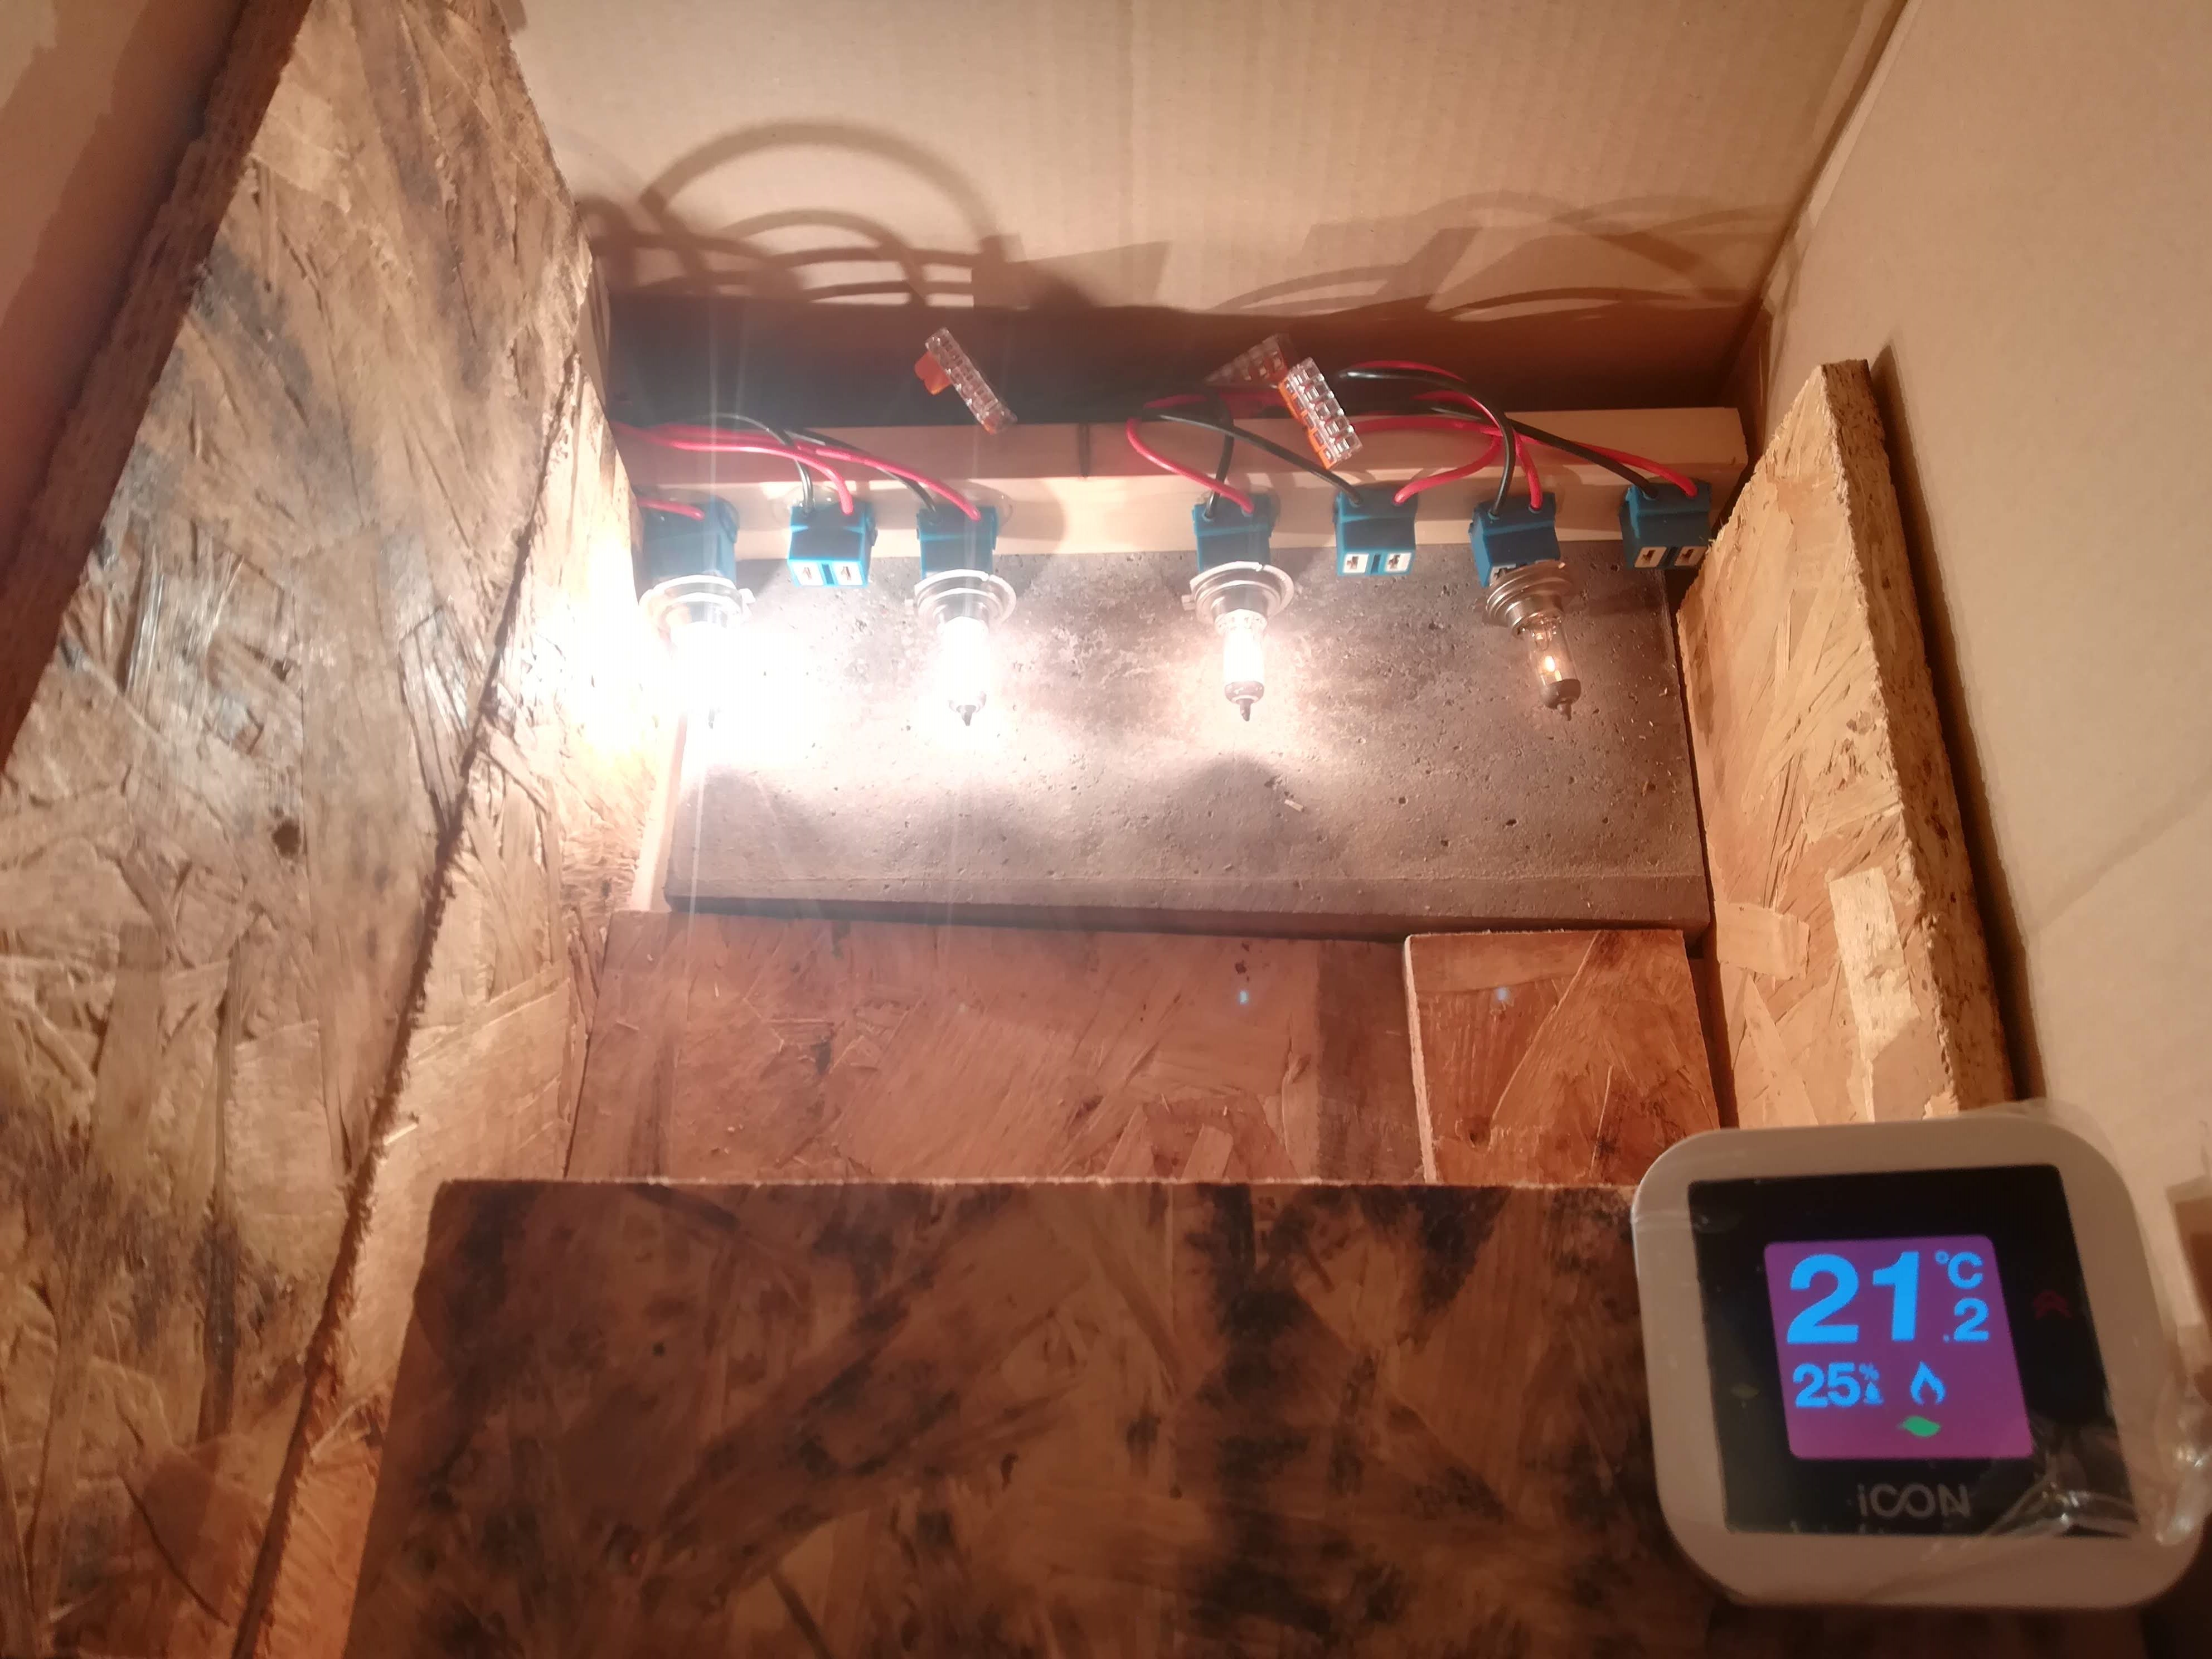
\includegraphics[width=0.8\textwidth]{figures/realsys/interior2}
	\caption{A doboz belseje hőmérővel és szabályozható izzókkal}
	\label{fig:realsys-interior}
\end{figure}

\section{A Simulink konfigurálása}
A valós idejű futáshoz Simulink  Real-time szükséges. A real-time működés itt azt jelenti, hogy a szabályozót a Simulink mintavételi időnként futtatja le. Azaz ha a kísérleti rendszerre \SI{30}{\second}-es mintavételi idejű szabályzót tervezek, akkor az MPC félpercenként mintát fog venni a hőmérsékletekből és ki fog adni egy beavatkozójelet. Így a real-time ez esetben nem jelent például szigorú korlátokat a futásidőre.


%A Real-time UDP-t használom. %https://uk.mathworks.com/help/xpc/io_ref/udp-transport-protocol.html
%https://uk.mathworks.com/products/simulink-desktop-real-time.html

A szabályzó a számítógépen fut, és mintavételi időnként a jelenlegi hőmérsékletet beolvassa, az MPC-t lefuttatja, a beavatkozó jeleket pedig elküldi a beágyazott számítógépnek.

\begin{figure}
	\centering
	\begin{tikzpicture}[>=stealth,
  		%inner/.style={draw,fill=blue!5,thick,inner sep=3pt,minimum width=8em},
		%outer/.style={draw=gray,dashed,fill=green!1,thick,inner sep=5pt}
		outer/.style={draw=gray,dashed,thick,inner sep=5pt}
		]
	
	% Szabályzási kör elemei
	% ----------------------
	
		% Szabályzó
		\node[draw,rectangle, minimum height=2cm,minimum width=6cm] (MPC) at (3.2,3.5) {\parbox{2cm}{\centering MPC szabályozás}};		

		% Fűtési rendszer
		\node[draw,rectangle, minimum height=1.6cm,minimum width=5cm] (Heat) at (7,0) {\parbox{2cm}{\centering iContrALL~~~~ \\ dimmer~~}};
	
		% Ház
		\node[draw,rectangle, minimum height=1.6cm,minimum width=3.2cm] (House) at (2,0) {helyiség modellje};
		
		% Hőmérő
		\node[draw,rectangle, minimum height=1.6cm,minimum width=3.2cm] (Measure) at (-2,0) {\parbox{2cm}{\centering hőmérséklet\\mérés}};
		
		%Zavarás
		\node[rectangle, minimum height=0.8cm,minimum width=2cm,below=of House, node distance=1cm] (ghostDist)  {Zavarás};

		
	
	% Kiegészítő cuccok
	% ----------------------
	
	% Keret - Matlab
	\node[draw,outer,rectangle, minimum height=4cm,minimum width=8cm,
	label={[label distance=-0.1cm, anchor=north]100:Simulink, számítógépen real-time fut}] (keret) at (3.2,3.5) {};
	
	% Zavarás a modellbemenetre
	\draw[->] (ghostDist.90) --  (House.270) node[above]{$T_e$};
	
	%\draw[->] (ctr.191) node[right]{${u_{2}}$} -| ++(-1.7,1.3)|-  (Numeric.172) node[right]{$\alpha_{floor}$};  %node[above left]{$\alpha_{radiator}$}; 
	
	% mért változók
	\draw[->] (House.180) -- (Measure.0);
	\draw[->] (Measure.195) node[right]{$T_e$} -| ++(-1.2,0)  |-  (MPC.168) node[right]{MD} ;
	\draw[->] (Measure.165) node[right]{${T_{i}}$}-| ++(-0.5,0.8)  |-  (MPC.188) node[right]{MO} ;

	
	%\draw[->] (d.0) node[left]{heat [W]} ->  ++(3,0) ->  (house.180);
	% Beavatkozó jel
	\draw [->] (MPC.0) node[left]{MV} -| ++(4,-2.5)  |- (Heat.0) node[left]{${u_1}$}; %++(1.5cm,0) -- (2cm,0pt) -- (2.5cm,10pt);
	
	\draw[->] (Heat.180)  node[right]{$Q_{ki}$} -- (House.0) ;
	%\draw[->] (d.20) -| ++(1,-1) |- (y.350);
	
	%\path 
	%(d.150)	 edge[<->] 	node[anchor=north,above]{valvePercent}	(y.270);
	
	% Lehetséges label beállítások:
		%label={[blue,yshift=0.3cm]above:Z}]
	
%	\node[draw,outer,rectangle, minimum height=5.5cm,minimum width=13cm,
%	label={[label distance=-0.1cm, anchor=north]270:3 bemenetű, 1 kimenetű szakaszmodell}] (keret) at (0,15) {};
%	
%	
	\end{tikzpicture}

	\caption{A valós idejű mérések szereplői}
	\label{fig:realtimesimulink}
\end{figure}

%\begin{tikzpicture}[>=stealth,remember picture]
%\node[draw,rectangle,inner sep=0.5cm] (y) at (0,0) {$A$};
%\node[draw] (d) at (0,2) {%
%%	\begin{tikzpicture}[remember picture]
%%	\matrix [matrix of math nodes] (mat)
%%	{
%%		B & \phantom{C}   \\
%%		\phantom{B} & C \\
%%	};
%%	\end{tikzpicture}
%%};
%%\draw[->,shorten >= 6pt] (y.west) -| ++(-1,1) |- (mat-1-1);
%%\draw[->,shorten >= 6pt] (y.west) -| ++(-0.8,1) |- (mat-2-1);
%%\draw[->] ($(mat-2-2)+(14pt,0)$) -| ++(0.8,-1) |- (y.east);
%%\draw[->] ($(mat-1-2)+(14pt,0)$) -| ++(1,-1) |- (y.east);
%\end{tikzpicture}




% 3600001117-es ID-jű, Raspberry Pi, IP címe fixen 192.168.0.108, 54321-es port.

%A PI SPI-n küld a rádióadónak.
%Rádiókommunikáció egyirányú.

\section{Szabályozótervezés az identifikált modellre}
Mivel a kísérleti rendszeremnek nincsen energetikai tanúsítványa, identifikáltam az ugrásválaszával (\ref{fig:realsys-ident}. ábra).

\begin{figure}
	\centering
	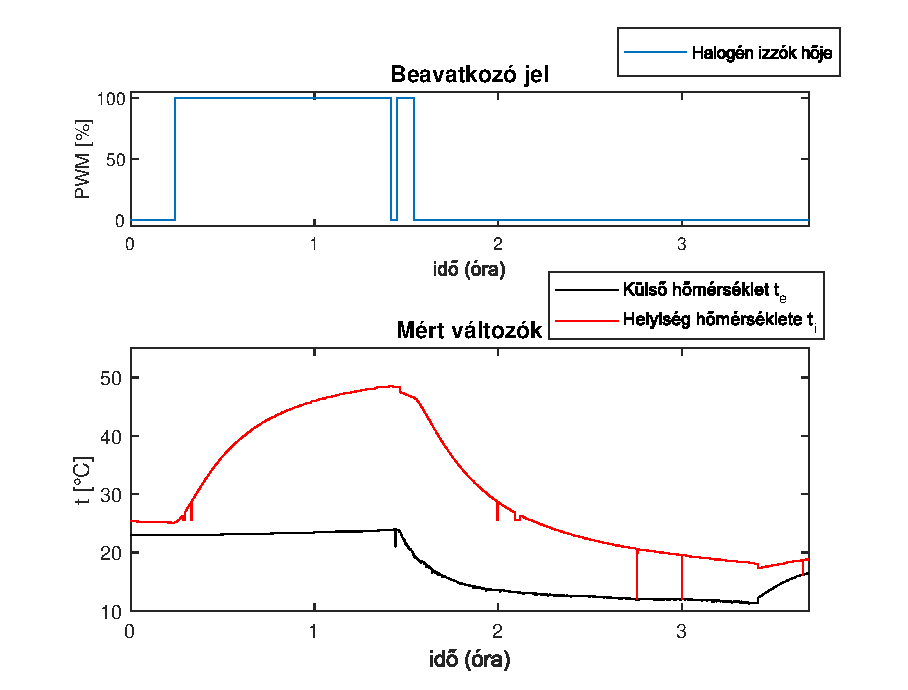
\includegraphics[width=0.65\textwidth]{figures/realsys/ident}
	\caption{Identfikációhoz használt mérési adatsor}
	\label{fig:realsys-ident}
\end{figure}

A valós idejű méréshez használni kívánt szabályozót érdemes először szimulációban megvizsgálni. Ekkor adott a szabályzott szakasz identifikált lineáris modellje, az MPC-t pedig létrehoztam  a modellhez az előző fejezet szerint. Az ott felmerülő nehézségeket, problémákat a fizikai rendszeren szerzett tapasztalatok miatt sikerült megoldani. A Simulinkben a tervezés a \textit{\ref{fig:mpc-sim}. ábra} szerinti elrendezésben történt, használva az MPC szabályozás közbeni (online) hangolásának lehetőségét.



\subsection{Mintavételi idő és predikciós horizont}

Az MPC paraméterezésére \textit{Agachi \cite{romanMPC_Agachi}} könyvében találhatók ajánlások. A predikciós horizontot eszerint úgy kell megválasztani, hogy az a szakasz releváns dinamikáját lefedje. Mivel a felfutási ideje a kísérleti rendszernek körülbelül 1 óra, ezért ezt ekkorára választottam. A predikciós horizont ajánlott nagysága 10-20 mintavétel a számítási igény csökkentése miatt (így $T_s =$ \SI{300}{\second} adódna),  viszont a mérés során gyakrabban szerettem volna látni a változásokat, a mintavételi időt 30 másodpercnek vettem.

\begin{figure}[h]
	\centering
	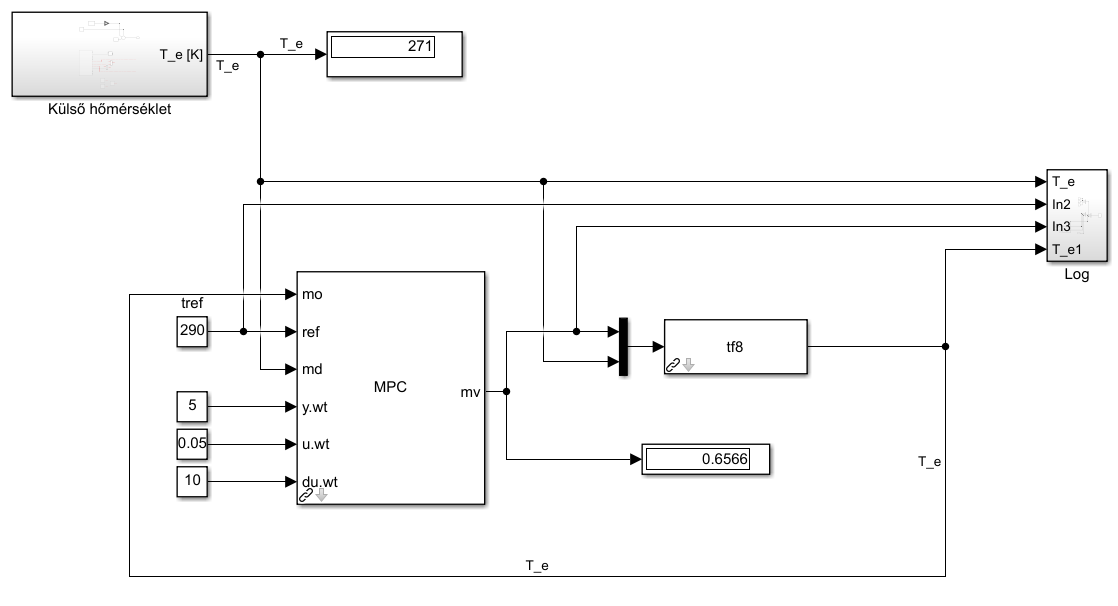
\includegraphics[width=\textwidth]{figures/simscape/simModel}
	\caption{Lineáris modellre MPC szimulációja}
	\label{fig:mpc-sim}
\end{figure}

A fentiek mellett viszont a szabályozó nem adott ki beavatkozójelet egészen egy predikciós horizontnyi ideig, azaz majdnem 1 órán keresztül\footnote{Ha 300 másodperces mintavételi időt használtam és 10 mintányi predikciós horizontot, ugyanez volt a helyzet. Ez idő alatt az MPC valószínűleg az állapotbecslőjét inicializálja.}. Az MPC képes a költségfüggvényben figyelembe venni a predikciós horizonton belül a referenciajel jövőbeli változásait (ez a \textit{Signal Previewing}), ezt kipróbáltam annak érdekében, hogy ezt a \say{holtidőt} csökkentsem, ám ellentétes hatást értem el.

A Simulink blokk viszont támogatja az MPC-nek kezdeti érték megadását. A kezdeti érték nélküli MPC-t szimulációban (azaz nem valós időben) futtattam, majd leolvastam annak belső állapotát. Az \verb|mpcstate| függvénnyel létre kellett hoznom egy objektumot, ami a Simulinkben a szabályzót inicializálja. Ehhez szükség volt a szabályzó állapotteres szakaszmodelljének\footnote{Amikor az MPC-t létrehozzuk, a szakaszmodellt a Matlab állapotteressé alakítja.} becsült állapotára, a zavarjel becsült értékére, a zaj becsült értékére (ez esetben üres vektor), a legutóbbi beavatkozójelre és egy kovarianciamátrixra (ezt nullmátrixnak vettem).

Azzal, hogy a fenti objektumban a legutóbbi beavatkozójelet maximálisnak vettem, valós idejű futás esetén, a fizikai rendszer ugrásválaszánál nem kellett kivárnom egy órát, azaz a predikciós horizontnyi időt, hanem a szabályzó rögtön maximális beavatkozójelet adott ki.

\subsection{A szabályozó költségfüggvénye}

A költségfüggvény súlyait iteratívan választottam ki. A paraméterek akár a szabályozó futása közben is módosíthatók, hatásuk azonnal látható. Először a referenciakövetést leginkább befolyásoló $w_y$ paramétert állítottam be.
 
\begin{figure}[H]
	\centering
	% trim={<left> <lower> <right> <upper>}
	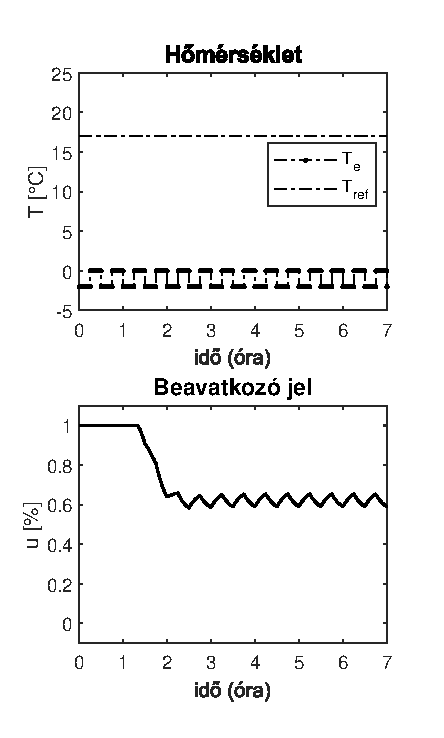
\includegraphics[width=0.4\textwidth, trim=0 168 0 0, clip,]{figures/realsys/disturbpar}
	\caption{Referenciajel és zavarás a szimuláció során}
	\label{fig:mpc-dist}
\end{figure}

\begin{figure}[H]
	\begin{subfigure}[t]{0.32\textwidth}
		\centering
		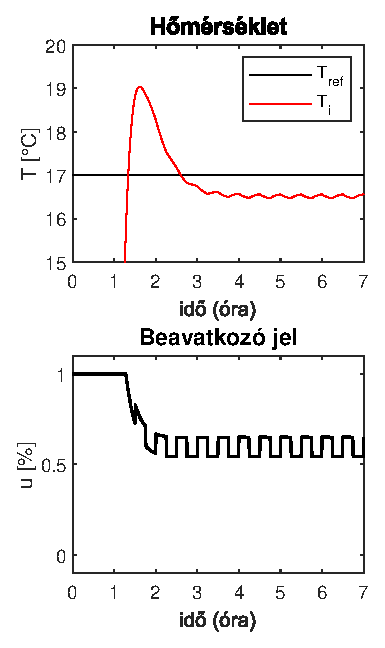
\includegraphics[width=\textwidth]{figures/realsys/mpc-wy-1}
		\caption{$w_y=1$}
		\label{fig:mpc-wy-1}
	\end{subfigure}
	~
	\begin{subfigure}[t]{0.32\textwidth}
		\centering
		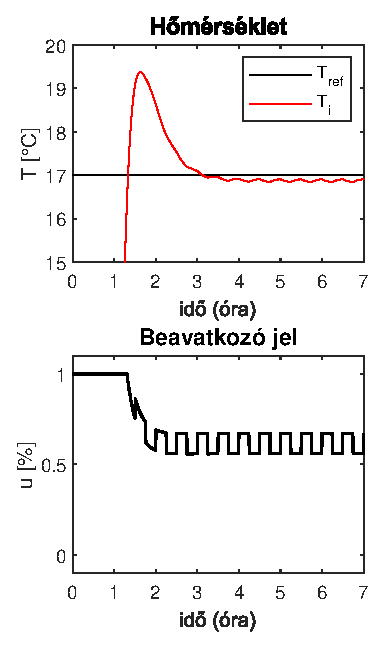
\includegraphics[width=\textwidth]{figures/realsys/mpc-wy-2}
		\caption{$w_y=2$}
		\label{fig:mpc-wy-2}
	\end{subfigure}
	~
	\begin{subfigure}[t]{0.32\textwidth}
		\centering
		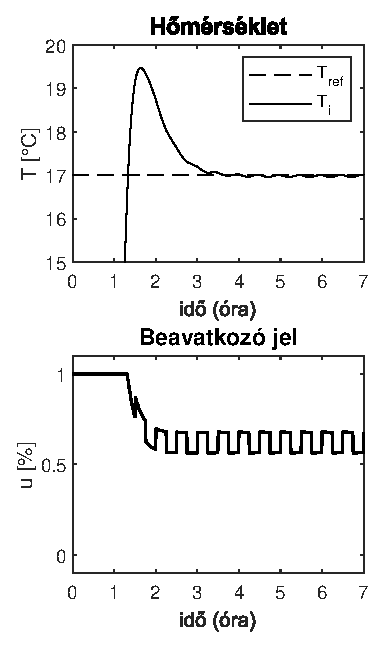
\includegraphics[width=\textwidth]{figures/realsys/mpc-wy-5}
		\caption{$w_y=5$}
		\label{fig:mpc-wy-5}
	\end{subfigure}
	\caption{MPC viselkedése különböző $w_y$ értékekre}
	\label{fig:mpc-wy}
\end{figure}

A \ref{fig:mpc-wy-5}.~ábrán látható esetben volt a legjobb a referenciakövetés, így ezt a paramétert rögzítettem. Következőnek a $w_u$ paraméter értékét választottam meg. Ez a beavatkozójel nagyságát bünteti.

\begin{figure}[H]
\begin{subfigure}[t]{0.32\textwidth}
	\centering
	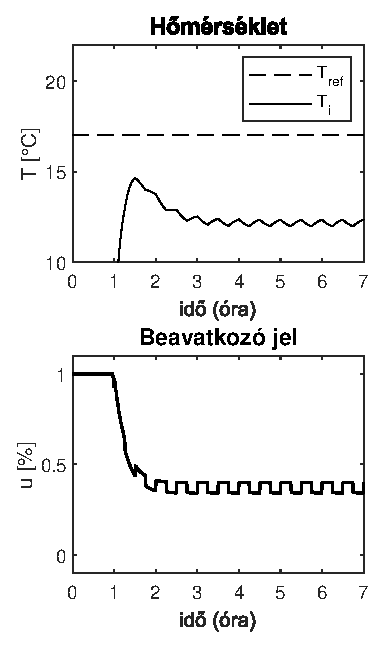
\includegraphics[width=\textwidth]{figures/realsys/mpc-wu-20}
	\caption{$w_u=20$}
	\label{fig:mpc-wu-20}
\end{subfigure}
~
\begin{subfigure}[t]{0.32\textwidth}
	\centering
	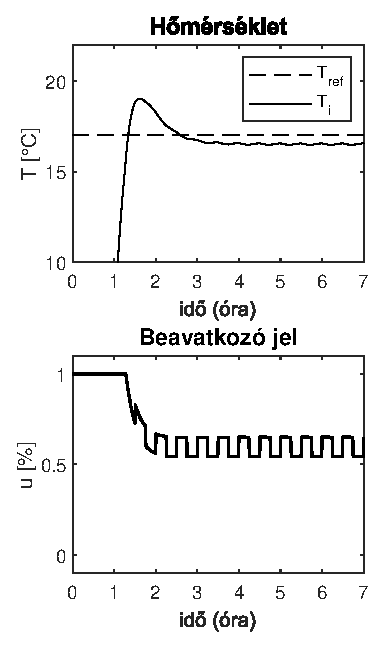
\includegraphics[width=\textwidth]{figures/realsys/mpc-wu-05}
	\caption{$w_u=5$}
	\label{fig:mpc-wu-05}
\end{subfigure}
~
\begin{subfigure}[t]{0.32\textwidth}
	\centering
	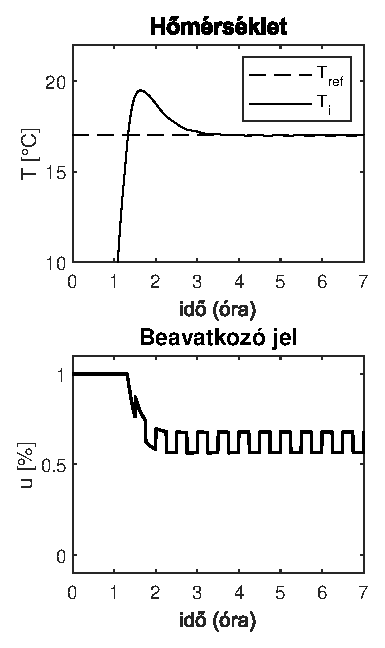
\includegraphics[width=\textwidth]{figures/realsys/mpc-wu-005}
	\caption{$w_u=0.05$}
	\label{fig:mpc-wu-005}
\end{subfigure}
\caption{MPC viselkedése különböző $w_u$ értékekre, $w_y=5$ mellett}
\label{fig:mpc-wu}
\end{figure}
 A \ref{fig:mpc-wu}.~ábrán látható, hogy nagy súly a költségfüggvényben lecsökkent beavatkozójelet, és így nagy követési hibát okoz. A két felsorolt paraméter valójában egymás ellenében hatnak\footnote{Bővebben a paraméterekről: https://uk.mathworks.com/help/mpc/ug/tuning-weights.html}.

A beavatkozást kevésbé büntettem, így a referenciakövetés megmaradt, viszont a túllövés lecsökkent. Most már két fix paraméter mellett választottam súlyt a beavatkozójel változási sebességéhez.

\begin{figure}[H]
\begin{subfigure}[t]{0.32\textwidth}
	\centering
	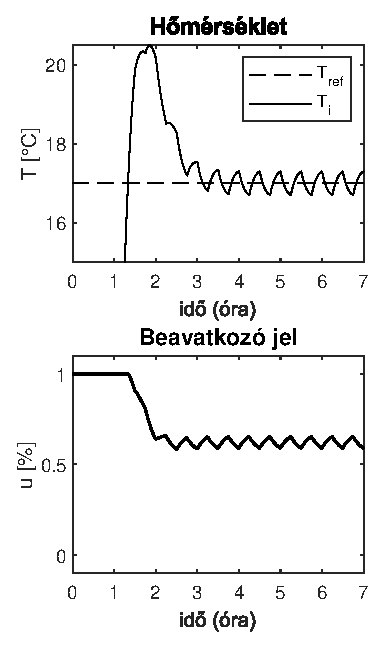
\includegraphics[width=\textwidth]{figures/realsys/mpc-wdu-100}
	\caption{$w_{\Delta u}=100$}
	\label{fig:mpc-wdu-100}
\end{subfigure}
~
\begin{subfigure}[t]{0.32\textwidth}
	\centering
	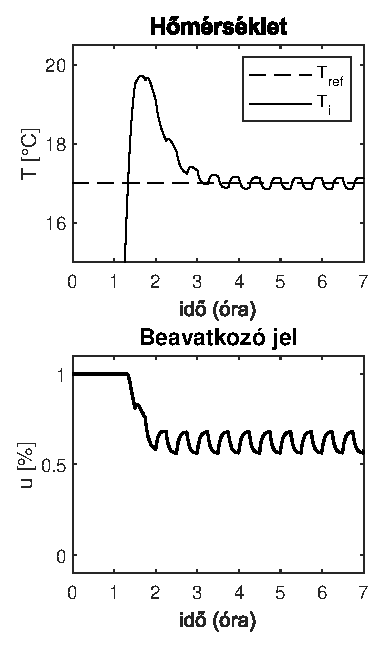
\includegraphics[width=\textwidth]{figures/realsys/mpc-wdu-50}
	\caption{$w_{\Delta u}=50$}
	\label{fig:mpc-wdu-50}
\end{subfigure}
~
\begin{subfigure}[t]{0.32\textwidth}
	\centering
	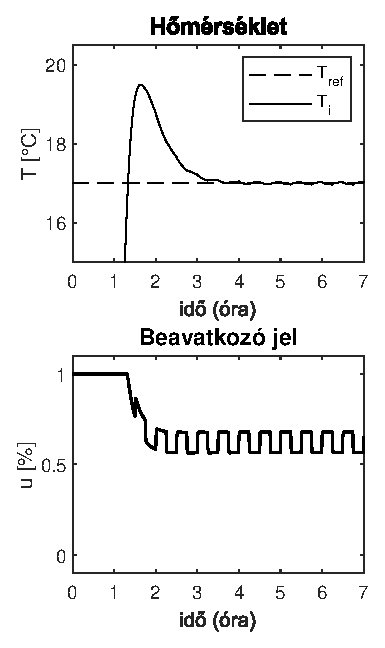
\includegraphics[width=\textwidth]{figures/realsys/mpc-wdu-10}
	\caption{$w_{\Delta u}=10$}
	\label{fig:mpc-wdu-10}
\end{subfigure}
\caption{MPC viselkedése  $w_{\Delta u}$ értékekre, $w_y=5$, $w_u=0.05$ mellett}
\label{fig:mpc-wdu}
\end{figure}

\begin{figure}[H]
	\centering
	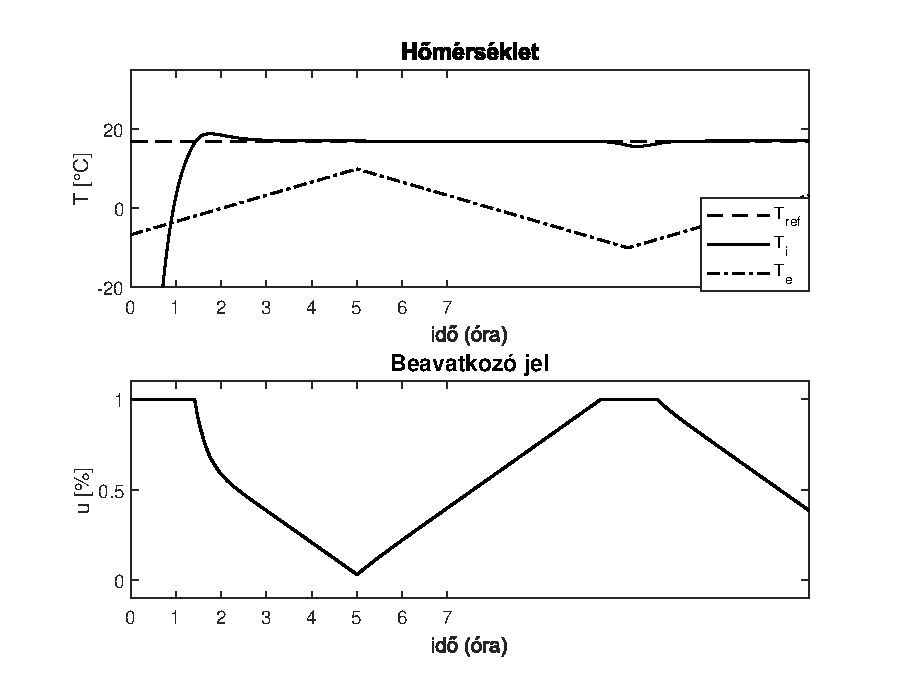
\includegraphics[width=0.7\textwidth]{figures/simscape/distrej}
	\caption{A zárt szabályozási kör ugrásválasza}
	\label{fig:mpc-distrej}
\end{figure}

A \ref{fig:mpc-wdu}. ábrán jól megfigyelhető, hogy nagy súly esetén a beavatkozójel frekvenciája lecsökken\footnote{A beavatkozás alapfrekvenciáját a \textit{\ref{fig:mpc-dist}. ábra} szerinti zavarjel adja, viszont a felfutás sebessége a $w_{\Delta u}$ paramétertől függ.}. Ez az épületgépészeti rendszerekben alacsonyabb energiafelhasználással járhat. Ám a három esetben különböző mértékű lengés tapasztalható állandósult állapotban: ezek közül az igényeknek, illetve a specifikációnak megfelelőt kell kiválasztani. A zavarelnyomást megvizsgáltam nagyobb tartományban változó külső hőmérséklettel is, ez látható a \textit{\ref{fig:mpc-distrej}. ábrán}.

A szabályzót kipróbáltam a kísérleti rendszeren is, a \textit{\ref{fig:realtimesimulink}. ábra} szerinti elrendezésben. A pontozott vonal a doboz környezeti hőmérséklete, a csökkenést az ablak kinyitásával értem el.
A külső hőmérséklet 85 perc környékén \SI{23}{\degreeCelsius}-ról csökkenni kezdett egészen \SI{8}{\degreeCelsius}-ra, de az MPC már a zavarás kezdetekor megnövelte a beavatkozó jelét és tartotta a referencia értéket. 

\begin{figure}[H]
	\centering
	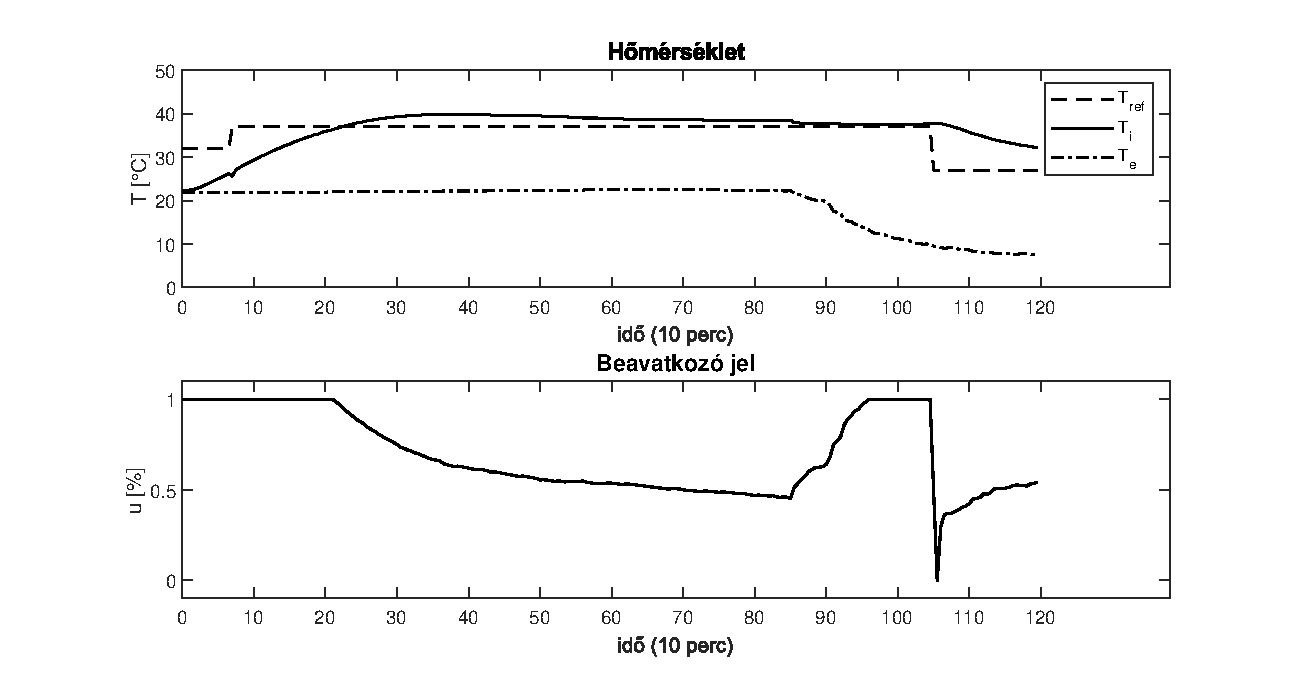
\includegraphics[width=0.95\textwidth]{figures/realsys/step}
	\caption{Mérés a fizikai rendszeren a behangolt MPC-vel}
	\label{fig:mpc-step}
\end{figure}

A tárgyaltakon felül további lehetőségek is vannak a költségfüggvények megadására. \textit{Thieblemont és Schirrer} \cite{SCHIRRER201686} megmutatta, hogy különösen jó eredmény érhető el MPC szabályozás és megújuló energiák kombinált használatával. A költségfüggvényekben például laza megkötéseket is lehet tenni, amik az adott jelet korlátozzák ugyan, de mégis túlléphetők - ilyenek egy napelemes rendszernél könnyen előfordulhatnak. Ekkor a laza felső korlát lehet a napelemes rendszer teljesítménye, de ezen felül is lehet energiát felhasználni a hálózatból.

Szintén \textit{Thieblemont} \cite{THIEBLEMONT2017485} készített felmérést az időjárás-előrejelzéssel kombinált MPC használatáról. (Itt a már korábban említett Signal Prevewing funkció használatos a jövőbeli bemenetek becsléséhez.) Az itt olvasható tapasztalatok és a bemutatott módszerek iránymutatást adhatnak a jövőbeni fejlesztésekhez.


%% Feljesztési lehetőségek
%\begin{formal}
%	Még lehetséges:
%	\begin{itemize}[noitemsep,topsep=-8pt,parsep=0pt,partopsep=0pt]
%		%		\item kazán bekapcsolása
%		%		\item előremenő hőmérséklet - unmeasured VAGY uncontrolled inputként
%		%		\item 1 db. fűtőtest (most radiátor) szelepének tömegárama (szelep áteresztése)
%		%		\item Később több fűtőtest vagy többféle fűtőtestek (padlófűtés, különböző teljesítményű radiátorok) szabályozása
%		\item környezeti hőmérséklet: predikció / szekvencia használata% is lesz rá. Hatása a kimeneten már identifikálva lett, 3 pólussal és 2 zérussal tökéletesen lekövethető.
%		\item napsugárzás zavaró hatása% - szimulálható  a bizonytalansága valószínűleg nagy lesz
%	\end{itemize}
%	
%	Belső változók - fűtési rendszer és ház kapcsolata
%	\begin{itemize}[noitemsep,topsep=-6pt,parsep=0pt,partopsep=0pt]
%		\item napsugárzás - radiatív, az ablak felületével és a szöggel arányos
%		\item fűtőtestek sugárzó és konvektív hőárama
%	\end{itemize}
%	
%	Paraméterek a plantben nem állandók:
%	\begin{itemize}[noitemsep,topsep=-6pt,parsep=0pt,partopsep=0pt]
%		%		\item hőátadási tényezők hőmérsékletfüggők, áramlási sebesség-függők (szél)
%		\item szellőztetés, belső hőterhelés hatása
%	\end{itemize}
%\end{formal}